\newpage
\section{图例}

矩形：\verb|rectangle|\quad 抛物线：\verb|parabola bend|

\begin{proset}
	
	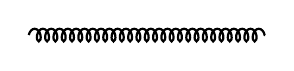
\begin{tikzpicture}
		% 弹簧
		\draw[thick,decoration={aspect=.6,segment length=3,amplitude=.8mm,coil},decorate] (0,0)--(3,0);
	\end{tikzpicture}	
\end{proset}

\begin{proset}
	
	\begin{tikzpicture}[decoration={markings,mark=at position 0.5 with {\arrow{>}}}]
		\draw[postaction={decorate},purple] (0,0)--(3,0);
	\end{tikzpicture}
\end{proset}

\begin{proset}
	斜面

	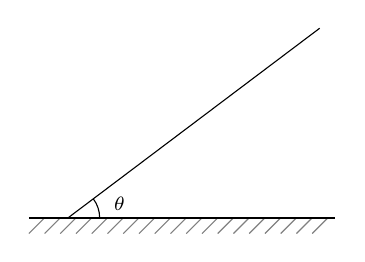
\begin{tikzpicture}[font=\scriptsize]
		\def\TheTa{37}%旋转角度
		\def\LenGth{4}%斜面长度
		\pgfmathsetmacro\CosLenGth{\LenGth*cos(\TheTa)}
		\begin{scope}[rotate=\TheTa]	
			\draw (0,0)--++(\LenGth,0);
		\end{scope}
		\draw (.4,0) arc(0:\TheTa:.4);
		\node at(.65,.18){\(\theta\)};
		\foreach \x in{-.5,-.3,...,\CosLenGth}
			\draw[gray] (\x,-.2)--++(.2,.2);
		\draw[thick] (-.5,0)--({\CosLenGth+.2},0);
	\end{tikzpicture}
\end{proset}

\begin{proset}
	弹簧测力计、立方体

	\begin{tikzpicture}
		\begin{scope}
			\coordinate (o) at(0,0);
			\draw ($(o)+(0,.3)$)--($(o)+(0,.12)$) arc(90:-180:.06);
			\draw ($(o)+(-.12,.42)$) arc(-180:0:.12)--++(.06,0)--++(0,1.72)--++(-.06,0) arc(0:180:.12)--++(-.06,0)--++(0,-1.72)--($(o)+(-.12,.42)$) ($(o)+(0,2.38)$) circle(.12) ($(o)+(0,2.38)$) circle(.08);
			\draw[fill=red!50,draw=white] ($(o)+(-.04,.5)$) rectangle($(o)+(.04,1.4)$);
			\draw[thin] ($(o)+(-.12,.5)$)--++(.24,0) ($(o)+(-.04,.5)$)--++(0,1.5) ($(o)+(.04,.5)$)--++(0,1.5) ($(o)+(-.12,2)$)--++(.24,0);
			\foreach \y in {.5,.8,...,2}
				\draw[thin] (-.04,\y)--++(-.08,0) (.04,\y)--++(.08,0);
		\end{scope}%%(0,0)(0,2.5)
		\begin{scope}[xshift=1cm]
			\coordinate (o)at(0,0);
			\draw (o) rectangle($(o)+(1,1)$)coordinate(b) (b)--++(45:{.5*sqrt(2)})coordinate(c)--++(-1,0)coordinate(d)--++(-135:{.5*sqrt(2)}) (c)--++(0,-1)--++(-135:{.5*sqrt(2)});
			\draw[dashed] (o)--++(45:{.5*sqrt(2)})--++(1,0) (d)--++(0,-1);
		\end{scope}
	\end{tikzpicture}
\end{proset}

\begin{proset}
	纸带

	\begin{tikzpicture}
		\coordinate (o) at(0,0);
		\draw ($(o)+(-.3,.5)$)--++(10.2,0) ($(o)+(-.3,-.5)$)--++(10.2,0)coordinate(a) ($(o)+(-.3,.5)$)--++(-.1,-.1)--++(.2,-.7)--++(-.1,-.2) (a)--++(.1,.1)--++(-.2,.7)--++(.1,.2);
		\node at($(a)+(-.7,-.2)$){\scriptsize 单位：\,\qty{}{cm}};
		\foreach \x/\n in {0/0,.6/1,1.6/2,3/3,4.8/4,7/5,9.6/6}{
			\coordinate (\n) at(\x,0);
			\draw[gray] (\x,.05)--++(0,.15);
			\fill (\n)node[below]{\scriptsize \(\n\)} circle(.03);}
		\foreach \x/\y/\n in {0/.6/0,.6/1.6/0,1.6/3/0,3/4.8/0,4.8/7/0,7/9.6/0}
			\draw[stealth-stealth,thin] (\x,.1)--node[above]{\scriptsize \(\n\)}(\y,.1);
	\end{tikzpicture}%%始.6,差.4

	\begin{tikzpicture}
		\coordinate (o) at(0,0);
		\draw ($(o)+(-.3,.5)$)--++(10.2,0) ($(o)+(-.3,-.5)$)--++(10.2,0)coordinate(a) ($(o)+(-.3,.5)$)--++(-.1,-.1)--++(.2,-.7)--++(-.1,-.2) (a)--++(.1,.1)--++(-.2,.7)--++(.1,.2);
		\node at($(a)+(-.7,1.2)$){\scriptsize 单位：\,\qty{}{cm}};
		\foreach \x/\n in {0/0,.6/1,1.6/2,3/3,4.8/4,7/5,9.6/6}{
			\coordinate (\n) at(\x,0);
			\fill (\n)node[above]{\scriptsize \(\n\)} circle(.03);}
		\foreach \y/\x/\n in {-.7/.6/2.78,-1.1/1.6/7.70,-1.5/3/12.86,-1.9/4.8/20.16,-2.3/7/28.95,-2.7/9.6/38.22}
			\draw[stealth-stealth,thin] (0,\y)--node[below]{\scriptsize \(\n\)}(\x,\y);
		\foreach \x/\y in {0/-2.8,.6/-.8,1.6/-1.2,3/-1.6,4.8/-2.0,7/-2.4,9.6/-2.8}
			\draw[gray] (\x,-.1)--(\x,\y);
	\end{tikzpicture}%%始.6,差.4
\end{proset}
\begin{proset}
	螺旋测微计
	
	\begin{tikzpicture}[scale=1.5]
		\coordinate (o) at(0,0);
		\coordinate (a) at(2.843,0);%%主尺长度调节
		\coordinate (d) at(0,.015);%%主尺上下调节值
		%主尺长度及上下微调
		\draw ($(o)+(-.2,0)+(d)$)--($(a)+(d)$);
		\foreach \x in {0,.2,.4,...,2.8}{
			\draw ($(\x,0)+(d)$)--++(0,-.25);
			\draw ($({\x+.1},0)+(d)$)--++(0,.2);}
		\foreach \x/\n in {0/0,1/5,2/10}
			\draw ($(\x,-.25)+(d)$)--++(0,-.15)node[below]{\scriptsize \(\n\)};
		%尺两端
		\draw ($(o)+(-.2,-.9)$)--($(a)+(0,-.9)$) ($(o)+(-.2,.9)$)--($(a)+(0,.9)$);
		\draw[fill=gray!15] ($(a)+(1.5,-1.1)$)--++(-.8,0)--++(-.2,.1)--++(-.5,.05)--++(0,1.9)--++(.5,.05)--++(.2,.1)--++(.8,0);
		\draw[fill=gray!25] ($(o)+(-.2,0)$)--++(0,1)--++(-.6,0)..controls($(o)+(-1.2,.5)$)and($(o)+(-.4,-.5)$)..($(o)+(-.8,-1)$)--++(.6,0)--++(0,1);
		\draw ($(o)+(-.8,-1)$)..controls($(o)+(-1,-.5)$)..($(o)+(-.8,0)$);
		%副尺刻度
		\foreach \y in {-.9,-.8,...,.8}
			\draw[blue,thin] ($(a)+(0,\y)$)--++(.2,0);
		\foreach \y/\n in {-.7/15,-.2/20,.3/25,.8/30}
			\draw[red,thin] ($(a)+(0,\y)$)--++(.3,0)node[right]{\scriptsize \(\n\)};
	\end{tikzpicture}
\end{proset}
\begin{proset}
	游标卡尺

	\begin{tikzpicture}[scale=1.5]
		\coordinate (o) at(0,0);
		\coordinate (length) at(3.3,0);%主尺长度
		\coordinate (d) at(1.14,0);%游标移动值
		%游标
		\draw[gray] ($(o)+(-.1,0)+(d)$) rectangle($(o)+(1.1,-.5)+(d)$);
		\foreach \x in {0,.09,...,.9}
			\draw[blue] ($(\x,0)+(d)$)--++(0,-.1);
		\foreach \x in {0,0.45,...,.9}
			\draw[blue] ($(\x,-.1)+(d)$)--++(0,-.05);
		\foreach \x/\n in {0/0,.45/5,.9/10}
			\draw[blue] ($(\x,-.15)+(d)$)--++(0,-.05)node[below]{\scriptsize \(\n\)};
		%主尺
		\foreach \x in {0,.1,...,3.3}
			\draw[blue] (\x,0)--++(0,.2);
		\foreach \x in {0,.5,...,3}
			\draw[blue] (\x,.2)--++(0,.05);
		\foreach \x/\n in{0/0,1/1,2/2,3/3}
			\draw[blue] (\x,.25)--++(0,.05)node[above]{\scriptsize \(\n\)};
		\draw ($(o)+(-.2,0)$)--(length);
		\node[blue] at(3.2,.3)[above]{\scriptsize \,\qty{}{cm}};
	\end{tikzpicture}

	\begin{tikzpicture}[scale=1.5]
		\coordinate (o) at(0,0);
		\coordinate (length) at(3.3,0);%主尺长度
		\coordinate (d) at(.24,0);%游标移动值
		%游标
		\draw[gray] ($(o)+(-.1,0)+(d)$) rectangle($(o)+(2.1,-.5)+(d)$);
		\foreach \x in {0,.095,...,1.91}
			\draw[blue] ($(\x,0)+(d)$)--++(0,-.1);
		\foreach \x in {0,0.475,...,1.91}
			\draw[blue] ($(\x,-.1)+(d)$)--++(0,-.05);
		\foreach \x/\n in {0/0,.95/10,1.9/20}
			\draw[blue] ($(\x,-.15)+(d)$)--++(0,-.05)node[below]{\scriptsize \(\n\)};
		%主尺
		\foreach \x in {-.1,0,.1,...,3.3}
			\draw[blue] (\x,0)--++(0,.2);
		\foreach \x in {0,.5,...,3}
			\draw[blue] (\x,.2)--++(0,.05);
		\foreach \x/\n in{0/1,1/2,2/3,3/4}
			\draw[blue] (\x,.25)--++(0,.05)node[above]{\scriptsize \(\n\)};
		\draw ($(o)+(-.2,0)$)--(length);
		\node[blue] at(3.2,.3)[above]{\scriptsize \,\qty{}{cm}};
	\end{tikzpicture}

	\begin{tikzpicture}[scale=1.5]
		\coordinate (o) at(0,0);
		\coordinate (length) at(6.5,0);%主尺长度
		\coordinate (d) at(1.044,0);%游标移动值
		%游标
		\draw[gray] ($(o)+(-.1,0)+(d)$) rectangle($(o)+(5.1,-.5)+(d)$);
		\foreach \x in {0,.098,...,4.91}
			\draw[blue] ($(\x,0)+(d)$)--++(0,-.12);
		\foreach \x/\n in {0/0,.49/1,.98/2,1.47/3,1.96/4,2.45/5,2.94/6,3.43/7,3.92/8,4.41/9,4.9/10}
			\draw[blue] ($(\x,-.12)+(d)$)--++(0,-.08)node[below]{\scriptsize \(\n\)};
		%主尺
		\foreach \x in {0,.1,...,6.4}
			\draw[blue] (\x,0)--++(0,.2);
		\foreach \x in {0,.5,...,6.4}
			\draw[blue] (\x,.2)--++(0,.05);
		\foreach \x in{0,1,...,6.4}
			\draw[blue] (\x,.25)--++(0,.05)node[above]{\scriptsize \(\x\)};
		\draw ($(o)+(-.2,0)$)--(length);
		\node[blue] at(6.2,.3)[above]{\scriptsize \,\qty{}{cm}};
	\end{tikzpicture}
\end{proset}
\begin{proset}
	传送带

	\begin{tikzpicture}
		\begin{scope}[rotate=37]
			\coordinate (o) at(0,0);
			\coordinate (length) at(3,0);
			\coordinate (square) at(0,.3);
			\draw[gray] (0,0) circle(.25) (length) circle(.25);
			\draw[fill=orange!50] (square) rectangle($(square)+(.3,.3)$);
			\draw[purple] ($(o)+(0,.3)$)--($(length)+(0,.3)$) arc(90:-90:.3)--($(length)+(0,-.3)$)--($(o)+(0,-.3)$) arc(270:90:.3);
			\fill (o) circle(.07) (length) circle(.07);
			\draw[-stealth] (1.2,.2)--node[below]{\footnotesize\(v_0\)}(2,.2);
		\end{scope}
		\draw[dashed,gray] (0,-.3)--(2,-.3);
		\draw[gray] ({.3*tan(18.5)+.4},-.3) arc(0:37:.4);
		\node at(.7,-.15){\footnotesize\(\theta\)};
	\end{tikzpicture}
\end{proset}
\begin{proset}
	电阻箱

	\begin{tikzpicture}
		\draw[rounded corners=10] (-.8,.9) rectangle(4,-3.2);
		\coordinate (a) at(3.7,-1.2);
		\draw ($(a)+(0,.25)$) circle(.15);
		\draw[fill=black] ($(a)+(0,.25)$) circle(.1);
		\draw[red] ($(a)+(0,-.25)$) circle(.15);
		\filldraw[fill=red,draw=red] ($(a)+(0,-.25)$) circle(.1);
		\begin{scope}
			\coordinate (o) at(0,0);
			\draw[blue] (o) circle(.6);
			\fill[gray!70!black] (0,0) circle(.22) ($(o)+(0,-.6)$)--++(-120:.25)--++(.25,0)--++(120:.25);
			\node at($(o)+(0,{-.6-.2*cos(30)})$)[below]{\scriptsize\(\times\:10\:\mathrm{k}\)};
			\foreach \x in {18,54,...,342}
				\draw (\x:.6)--(\x:.51);
			\foreach \x/\y/\n in {18/-72/7,54/-36/6,90/0/5,126/36/4,162/72/3,198/108/2,234/144/1,270/180/0,306/216/9,342/252/8}
				\node[purple] at(\x:.36){\tiny\rotatebox{\y}{\n}};
		\end{scope}
		\begin{scope}[xshift=1.4cm]
			\coordinate (o) at(0,0);
			\draw[blue] (o) circle(.6);
			\fill[gray!70!black] (0,0) circle(.22) ($(o)+(0,-.6)$)--++(-120:.25)--++(.25,0)--++(120:.25);
			\node at($(o)+(0,{-.6-.2*cos(30)})$)[below]{\scriptsize\(\times\:1\:\mathrm{k}\)};
			\foreach \x in {18,54,...,342}
				\draw (\x:.6)--(\x:.51);
			\foreach \x/\y/\n in {18/-72/7,54/-36/6,90/0/5,126/36/4,162/72/3,198/108/2,234/144/1,270/180/0,306/216/9,342/252/8}
				\node[purple] at(\x:.36){\tiny\rotatebox{\y}{\n}};
		\end{scope}
		\begin{scope}[xshift=2.8cm]
			\coordinate (o) at(0,0);
			\draw[blue] (o) circle(.6);
			\fill[gray!70!black] (0,0) circle(.22) ($(o)+(0,-.6)$)--++(-120:.25)--++(.25,0)--++(120:.25);
			\node at($(o)+(0,{-.6-.2*cos(30)})$)[below]{\scriptsize\(\times\:100\)};
			\foreach \x in {18,54,...,342}
				\draw (\x:.6)--(\x:.51);
			\foreach \x/\y/\n in {18/-72/7,54/-36/6,90/0/5,126/36/4,162/72/3,198/108/2,234/144/1,270/180/0,306/216/9,342/252/8}
				\node[purple] at(\x:.36){\tiny\rotatebox{\y}{\n}};
		\end{scope}
		\begin{scope}[xshift=0cm,yshift=-1.8cm]
			\coordinate (o) at(0,0);
			\draw[blue] (o) circle(.6);
			\fill[gray!70!black] (0,0) circle(.22) ($(o)+(0,-.6)$)--++(-120:.25)--++(.25,0)--++(120:.25);
			\node at($(o)+(0,{-.6-.2*cos(30)})$)[below]{\scriptsize\(\times\:10\)};
			\foreach \x in {18,54,...,342}
				\draw (\x:.6)--(\x:.51);
			\foreach \x/\y/\n in {18/-72/7,54/-36/6,90/0/5,126/36/4,162/72/3,198/108/2,234/144/1,270/180/0,306/216/9,342/252/8}
				\node[purple] at(\x:.36){\tiny\rotatebox{\y}{\n}};
		\end{scope}
		\begin{scope}[xshift=1.4cm,yshift=-1.8cm]
			\coordinate (o) at(0,0);
			\draw[blue] (o) circle(.6);
			\fill[gray!70!black] (0,0) circle(.22) ($(o)+(0,-.6)$)--++(-120:.25)--++(.25,0)--++(120:.25);
			\node at($(o)+(0,{-.6-.2*cos(30)})$)[below]{\scriptsize\(\times\:1\)};
			\foreach \x in {18,54,...,342}
				\draw (\x:.6)--(\x:.51);
			\foreach \x/\y/\n in {18/-72/7,54/-36/6,90/0/5,126/36/4,162/72/3,198/108/2,234/144/1,270/180/0,306/216/9,342/252/8}
				\node[purple] at(\x:.36){\tiny\rotatebox{\y}{\n}};
		\end{scope}
		\begin{scope}[xshift=2.8cm,yshift=-1.8cm]
			\coordinate (o) at(0,0);
			\draw[blue] (o) circle(.6);
			\fill[gray!70!black] (0,0) circle(.22) ($(o)+(0,-.6)$)--++(-120:.25)--++(.25,0)--++(120:.25);
			\node at($(o)+(0,{-.6-.2*cos(30)})$)[below]{\scriptsize\(\times\:0.1\)};
			\foreach \x in {18,54,...,342}
				\draw (\x:.6)--(\x:.51);
			\foreach \x/\y/\n in {18/-72/7,54/-36/6,90/0/5,126/36/4,162/72/3,198/108/2,234/144/1,270/180/0,306/216/9,342/252/8}
				\node[purple] at(\x:.36){\tiny\rotatebox{\y}{\n}};
		\end{scope}
	\end{tikzpicture}
\end{proset}
\begin{proset}
	桌子滑轮(pulley)

	\begin{tikzpicture}
		\coordinate (o) at(0,0);
		\draw[fill=orange!50] ($(o)+(-3.5,0)$)--(o)--++(0,-.2)--++(-3.5,0) ($(o)+(-.3,-.2)$)coordinate(a) rectangle($(a)+(-.3,-1.5)$);
		\draw[fill=orange!30] ($(o)+(-3.5,-.2)$)--($(a)+(-.3,0)$)--++(0,-.15)--($(o)+(-3.5,-.35)$);
		\draw[fill=blue!30] (-2.6,0)coordinate(b) rectangle($(b)+(-.4,.4)$);
		%%滑轮钩码
		\draw[thick] ($(o)+(.2,.1)$)coordinate(pulley) circle(.1) (o)--(pulley);
		\fill (pulley) circle(.05);
		\coordinate (pail) at($(pulley)+(.1,-1)$);
		\draw[purple] ($(b)+(0,.2)$)--($(pulley)+(0,.1)$) ($(pulley)+(.1,0)$)--($(pail)+(0,.11)$);
		\draw (pail)--++(0,.05) arc(-90:180:.03) ($(pail)+(0,-.1)$)--++(0,-.05) arc(90:360:.03);
		\draw[fill=gray!50] ($(pail)+(-.1,0)$) rectangle($(pail)+(.1,-.1)$);
		\draw[gray] ($(pail)+(0,-.05)$)--++(.5,0)node[right]{\scriptsize 钩码};
		\node at($(b)+(-.2,.4)$)[above]{\scriptsize \(P\)};
	\end{tikzpicture}
\end{proset}

\begin{proset}
	\begin{tikzpicture}[decoration={bumps,segment length=4mm,amplitude=1.2mm}]
		\draw[blue] (0,0)--(2,0)--(2,.4) (2,1.5)--(2,2)--(0,2) (2.4,1.6)--(2.4,2)--(4.4,2) (4.4,0)--(2.4,0)--(2.4,.4);
		\draw (0,-.1) rectangle(-.5,2.1) node[pos=.5]{\scriptsize\rotatebox{-90}{光伏电站}} (4.4,-.1) rectangle(4.9,2.1) node[pos=.5]{\scriptsize\rotatebox{90}{变电站}};
		\draw[fill=white] (3,-.1) rectangle(3.8,.1)node[pos=.5,above]{\scriptsize \(R\)};
		\draw[gray] (3,2)--(3.3,2.2)node[right]{\scriptsize 输电线};
		\draw[gray] (2.2,1.8)--(2.1,2.2)node[left]{\scriptsize 变压器};
		\draw[decorate,blue] (2,1.5)--(2,.3);
		\draw[decorate,blue] (2.4,.4)--(2.4,1.6);
	\end{tikzpicture}
\end{proset}

\begin{proset}

	\begin{tikzpicture}
        \draw[blue] (0,0) rectangle(3,2) (0,1)--(3,1);
        \draw[fill=white] (.5,0) circle(.15)node{\( \times \)}node[above right,font=\scriptsize]{\(D_1\)};\draw[fill=white] (1.5,1) circle(.15)node{\( \times \)}node[above right,font=\scriptsize]{\(D_2\)};\draw[fill=white] (2.5,2) circle(.15)node{\( \times \)}node[above right,font=\scriptsize]{\(D_3\)};
		%%% 电池
        \draw[fill=white,draw=white] (1.45,.-.2)coordinate(battery) rectangle ($(battery)+(.1,.4)$);
        \draw[blue] ($(battery)+(0,.4)$)--++(0,-.4) ($(battery)+(.1,.3)$)--++(0,-.2);
		%%% 开关
		\draw[fill=white,draw=white] (2,-.2)coordinate(switch) rectangle ($(switch)+(.45,.2)$);
        \draw[blue] ($(switch)+(0,.2)$) circle(.05) ($(switch)+(0,.25)$)--++(5:.5)node[above left,font=\scriptsize,black]{\(S\)};
    \end{tikzpicture}	
\end{proset}

\begin{proset}
	
	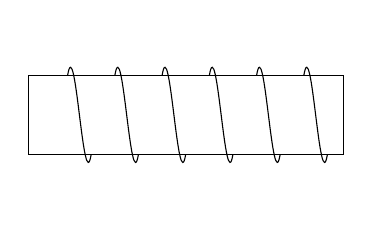
\begin{tikzpicture}
		\draw (0,0) rectangle(4,1);
		\foreach \x in{.5,1.1,...,4}
			\draw (\x,1)..controls({\x+.1},1.6)and({\x+.2},-.6)..({\x+.3},0);
	\end{tikzpicture}	
\end{proset}

\begin{proset}

	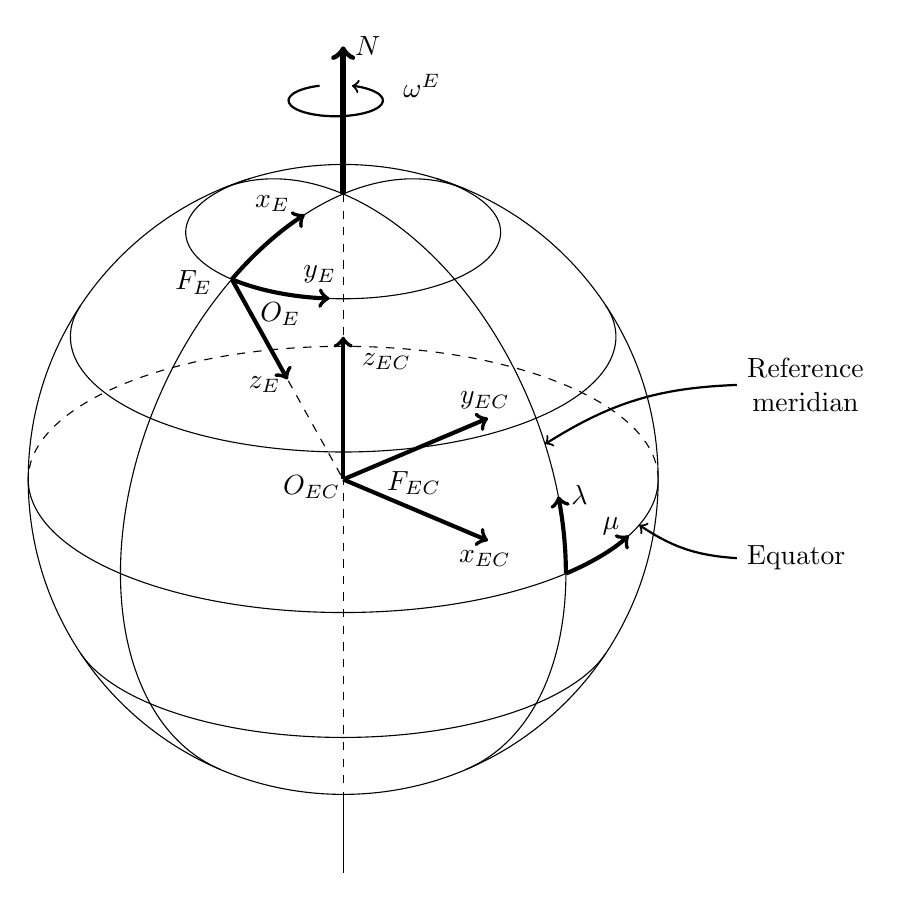
\begin{tikzpicture}
		\def\R{4}    % Spherical radius
		\def\AngleGamma{25}  % 极点倾斜角
		\pgfmathsetmacro\CosGamma{cos(\AngleGamma)} % pgfmathsetmacro 可以进行 cos 计算，def 不行
		\draw (0,0) circle (\R);
		
		\draw[->, very thick, line width=2pt] (0,\R*\CosGamma) to (0,5.5)node[right]{$N$};
		\draw[->,thick] (-0.3,5) arc [start angle=-250, end angle=70, x radius=0.6, y radius=0.2];
		\node at (1,5){$\omega^E$};
		
		\draw[dashed] (0,\R*\CosGamma) to (0,-4);
		\draw (0,-4) to (0,-5);
		\draw[->, thick, line width=1.5pt] (0, 0) to (0, 0.5*\R*\CosGamma);
		
		%% Longitude
		% Visibale angle
		\def\AngleLambda{45}
		\pgfmathsetmacro\LongiTemp{tan{\AngleGamma} / sin(\AngleLambda)}
		\pgfmathsetmacro\LongiVAngle{0.5 * atan(2 / (\LongiTemp - 1/\LongiTemp))}
		\draw[cm={cos(\AngleLambda), sin(\AngleGamma)*sin(\AngleLambda), 0, cos(\AngleGamma), (0,0)}] (\LongiVAngle + 90:\R) arc (\LongiVAngle + 90:\LongiVAngle+270:\R);
		% Markings
		\draw[dashed, cm={cos(\AngleLambda), sin(\AngleGamma)*sin(\AngleLambda), 0, cos(\AngleGamma), (0,0)}] (-0.5*\R, 0.866*\R) to (0,0);
		\draw[->, thick, line width=1.5pt, cm={cos(\AngleLambda), sin(\AngleGamma)*sin(\AngleLambda), 0, cos(\AngleGamma), (0,0)}] (-0.5*\R, 0.866*\R) to (-0.25*\R, 0.433*\R);
		\draw[->, thick, line width=1.5pt, cm={cos(\AngleLambda), sin(\AngleGamma)*sin(\AngleLambda), 0, cos(\AngleGamma), (0,0)}] (-0.5*\R, 0.866*\R) arc (120:100:\R);
		\draw[->, thick, line width=1.5pt, cm={cos(\AngleLambda), sin(\AngleGamma)*sin(\AngleLambda), 0, cos(\AngleGamma), (0,0)}] (0, 0) to (0.65*\R,0);
		
		\def\AngleLambda{135}
		\pgfmathsetmacro\LongiTemp{tan{\AngleGamma} / sin(\AngleLambda)}
		\pgfmathsetmacro\LongiVAngle{0.5 * atan(2 / (\LongiTemp - 1/\LongiTemp))}
		\draw[cm={cos(\AngleLambda), sin(\AngleGamma)*sin(\AngleLambda), 0, cos(\AngleGamma), (0,0)}] (\LongiVAngle + 90:\R) arc (\LongiVAngle + 90:\LongiVAngle+270:\R);
		% Markings
		\draw[->, thick, line width=1.5pt, cm={cos(\AngleLambda), sin(\AngleGamma)*sin(\AngleLambda), 0, cos(\AngleGamma), (0,0)}] (0, 0) to (-0.65*\R,0);
		\draw[->, thick, line width=1.5pt, cm={cos(\AngleLambda), sin(\AngleGamma)*sin(\AngleLambda), 0, cos(\AngleGamma), (0,0)}] (-\R, 0) arc (180:165:\R);
		
		
		%% Latitude
		\def\AngleAlpha{60}
		\pgfmathsetmacro\RAlpha{\R * cos(\AngleAlpha)}
		\pgfmathsetmacro\Yshift{\R * sin(\AngleAlpha) * cos(\AngleGamma)}
		\pgfmathsetmacro\LatiVAngle{asin(tan(\AngleAlpha) * tan(\AngleGamma))}
		\draw[cm={1, 0, 0, sin(\AngleGamma), (0,\Yshift)}] (180 - \LatiVAngle:\RAlpha) arc (180 - \LatiVAngle:360 + \LatiVAngle:\RAlpha);
		% Markings
		\draw[->, thick, line width=1.5pt, cm={1, 0, 0, sin(\AngleGamma), (0,\Yshift)}] (225:\RAlpha) arc (225:265:\RAlpha);
		
		\def\AngleAlpha{30}
		\pgfmathsetmacro\RAlpha{\R * cos(\AngleAlpha)}
		\pgfmathsetmacro\Yshift{\R * sin(\AngleAlpha) * cos(\AngleGamma)}
		\pgfmathsetmacro\LatiVAngle{asin(tan(\AngleAlpha) * tan(\AngleGamma))}
		\draw[cm={1, 0, 0, sin(\AngleGamma), (0,\Yshift)}] (180 - \LatiVAngle:\RAlpha) arc (180 - \LatiVAngle:360 + \LatiVAngle:\RAlpha);
		
		\def\AngleAlpha{0}
		\pgfmathsetmacro\RAlpha{\R * cos(\AngleAlpha)}
		\pgfmathsetmacro\Yshift{\R * sin(\AngleAlpha) * cos(\AngleGamma)}
		\pgfmathsetmacro\LatiVAngle{asin(tan(\AngleAlpha) * tan(\AngleGamma))}
		\draw[cm={1, 0, 0, sin(\AngleGamma), (0,\Yshift)}] (180 - \LatiVAngle:\RAlpha) arc (180 - \LatiVAngle:360 + \LatiVAngle:\RAlpha);
		\draw[dashed, cm={1, 0, 0, sin(\AngleGamma), (0,\Yshift)}] (0 - \LatiVAngle:\RAlpha) arc (0 - \LatiVAngle:180 + \LatiVAngle:\RAlpha);
		% Markings
		\draw[->, thick, line width=1.5pt, cm={1, 0, 0, sin(\AngleGamma), (0,\Yshift)}] (315:\RAlpha) arc (315:335 + \LatiVAngle:\RAlpha);
		
		
		\def\AngleAlpha{-30}
		\pgfmathsetmacro\RAlpha{\R * cos(\AngleAlpha)}
		\pgfmathsetmacro\Yshift{\R * sin(\AngleAlpha) * cos(\AngleGamma)}
		\pgfmathsetmacro\LatiVAngle{asin(tan(\AngleAlpha) * tan(\AngleGamma))}
		\draw[cm={1, 0, 0, sin(\AngleGamma), (0,\Yshift)}] (180 - \LatiVAngle:\RAlpha) arc (180 - \LatiVAngle:360 + \LatiVAngle:\RAlpha);
		
		% Markings
		\draw[->, thick] (5, 1.2)node[right, align=center]{Reference\\meridian} to[bend right=15] (2.5634, 0.4487);
		\draw[->, thick] (5, -1)node[right]{Equator} to[bend left=15] (3.7588, -0.5782);
		
		\node at (-0.4,-0.1){$O_{EC}$};
		\node at (0.9,-0.05){$F_{EC}$};
		\node at (1.8,-1){$\boldsymbol{x}_{EC}$};
		\node at (1.8,1){$\boldsymbol{y}_{EC}$};
		\node at (0.55,1.5){$\boldsymbol{z}_{EC}$};
		
		\node at (-1.9,2.5){$F_E$};
		\node at (-0.8,2.1){$O_E$};
		\node at (-0.9,3.5){$\boldsymbol{x}_E$};
		\node at (-0.3,2.6){$\boldsymbol{y}_E$};
		\node at (-1,1.2){$\boldsymbol{z}_E$};
		
		\node at (3.4,-0.6){$\boldsymbol{\mu}$};
		\node at (3, -0.2){$\boldsymbol{\lambda}$};
		\end{tikzpicture}
\end{proset}